% Diese Zeile bitte -nicht- aendern.
\documentclass[course=erap]{aspdoc}
\usepackage{subfig}
\usepackage{pgfplots}

\pgfplotsset{width = 10cm, compat = 1.9}
%%%%%%%%%%%%%%%%%%%%%%%%%%%%%%%%%
%% TODO: Ersetzen Sie in den folgenden Zeilen die entsprechenden -Texte-
%% mit den richtigen Werten.
\newcommand{\theGroup}{158} % Beispiel: 42
\newcommand{\theNumber}{A205} % Beispiel: A123
\author{Arda Mat \and Barış Özgün \and Yiğit Odakır}
\date{Sommersemester 2023} % Beispiel: Wintersemester 2019/20
%%%%%%%%%%%%%%%%%%%%%%%%%%%%%%%%%

% Diese Zeile bitte -nicht- aendern.
\title{Gruppe \theGroup{} -- Abgabe zu Aufgabe \theNumber}

\begin{document}
    \maketitle

    \section{Einleitung}\label{sec:einleitung}

    Die Aufgabenstellung befasst sich mit der Vergrößerung eines Fensters in einem
    unkomprimierten BMP-Bildformat für 24-Bit-Farbtiefe.
    Das Ziel ist also einen
    Schnitt des ursprünglichen Bildfensters auszuschneiden und folglich auszubreiten.

    Dementsprechend werden die vorhandenen Pixel auf ihren neuen Positionen verschoben
    und der Rest des Fensters wird mit geeigneten Pixeln gefüllt.
    Dafür wird eine Pixelwiederholungsmethode
    nämlich Nearest Neighbor~\cite{imageScalingAlgorithms} verwendet, die es ermöglicht,
    mathematische Konzepte in realen Anwendungen zu visualisieren~\cite{nearestNeighborInterpolation}.

    Dabei wird theoretisches mathematisches Wissen über das BMP-Format gebraucht um einen Algorithmus zur
    Manipulation von Bitfeldern zu entwickeln.
    Das Bitmap-Format wird häufig in der Praxis von Digitalkameras
    zur Speicherung von Pixelgrafiken verwendet.
    Die BMP-Dateien können komplexe Bilder in hoher Qualität speichern.
    Die Informationen über die Pixel sind in einem Pointer auf die sequentiellen Bilddaten gespeichert.
    Die Höhe, Breite und Größe der BMP-Datei, der Offset, wo das Pixelarray gefunden werden kann, die Druckauflösung des Bildes usw.
    können alle in der BMP-Datei gefunden werden~\cite{typesOfBitmaps}.

    Im theoretischen Teil dieses Projekts wird dafür gesorgt, dass das Rahmenprogramm Bildköpfe analysieren und relevante
    Metadaten, wie den Beginn der Pixeldaten sowie die Höhe und Breite des Bildes, zuverlässig identifizieren kann.
    Dementsprechend wird in diesem Projekt mit der Laufzeitanalyse des Algorithmus beschäftigt.
    Dafür wird ein Algorithmus für Eingabebilder aus 24-Bit-Pixeln entwickelt
    und die Laufzeit ungefähr durch die O-Notation beschrieben.

    Um die richtige Ausführung der Aufgabe sicherzustellen, werden
    I/O-Operationen in C implementiert, sodass die BMP-Datei eingelesen wird und sowohl die Bilddaten als auch die Metadaten
    wie die Breite, Höhe und Startadresse des Pixelarrays, an die C-Funktion übergeben werden können.
    Im Anschluss daran wird eine neue BMP-Datei konstruiert, indem die im Algorithmus berechneten
    Daten in diesem Datei-Format abgespeichert werden können.
    Als Ergebnis des Programms kann das neue Pixelbild betrachtet werden.

    In der Implementierung werden zwei Funktionen entwickelt: window() und zoom().
    Die window()-Methode schneidet aus den gegebenen Eingabedaten des Bildes ein Fenster aus
    und legt nur den Teil der Pixelkoordinaten im gewünschten Bereich (von den (x,y)-Koordinaten
    bis (x + width, y + height)-Koordinaten) in einem separaten Pufferspeicher abzu.
    Hingegen nimmt die zoom()-Methode das Ergebnis der window()-Methode, skaliert die Pixelwerte
    des Bildausschnitts bezüglich eines gegebenen Skalierungsfaktors und speichert die
    skalierten Bilddaten in einem resultierenden Pufferspeicher.

    Das Rahmenprogramm nimmt bei einem Aufruf verschiedene Optionen entgegen und verarbeitet.
    Man kann die verwendete Implementierung wählen, die Laufzeit der Implementierung messen
    und Werte für die Breite, Höhe des Fensters und den Skalierungsfaktor angeben.
    Das Rahmenprogramm behandelt fehlerhafte Eingaben korrekt.
    Im Auftritt eines Fehlers gibt das Programm eine aussagekräftige Fehlermeldung aus
    und bietet dem Benutzer eine kurze Erläuterung zur korrekten Verwendung des Programms.

    \section{Lösungsansatz}

    Das BMP-Bildformat wird um Bilder geräteunabhängig zu speichern verwendet.
    Meist benutzt sind die BMP-Dateien mit einer 24-Bit-Farbtiefe.
    Das heißt, dass ein Pixel aus 3 Bytes, die im RGB-Format liegen, besteht.
    Einerseits können Bilder mithilfe des BMP-Bildformats ohne Qualitätsverlust gespeichert werden.
    Auf der anderen Seite sind sie meist unkomprimiert und benötigen daher viel Speicherplatz.

    Jede BMP-Datei enthält 3 Teile: den Dateikopf, den Informationsblock und den Bilddaten. Der Dateikopf ist 14 Byte lang und gibt
    die Größe der BMP-Datei sowie den Offset der Pixel an. Der Informationsblock besteht aus 40 Bytes und enthält Informationen wie
    die Breite und Höhe des Bildes. In der unteren Tabelle kann man die wichtigsten Metadaten mit deren korrespondierenden Bytes
    in der Datei sehen. Diese Informationen sind wichtig, da damit das Programm diese Metadaten von der Datei auslesen und am Ende wieder
    eine gültige BMP-Datei erstellen kann.


    \begin{center}
        \begin{tabular}{| l | l  |}
            \hline
            Bytenummer & Daten \\ \hline
            2-3-4-5 & Größe der Datei in Bytes \\ \hline
            10-11-12-13 & Startbyte der Pixel  \\ \hline
            14-15-16-17 & Größe des Infoblocks \\ \hline
            18-19-20-21 & Breite der Pixeldatei (vorzeichenbehaftet) \\ \hline
            22-23-24-25 & Höhe der Pixeldatei (vorzeichenbehaftet) \\ \hline
            28-29 & Farbtiefe vom Bild \\ \hline
            38-39-40-41 & Horizontale Auflösung des Bildes \\ \hline
            42-43-44-45 & Vertikale Auflösung des Bildes \\ \hline
        \end{tabular}
    \end{center}


    An dieser Stelle ist es wichtig zu erwähnen, dass jede Reihe von Pixeln ein Alignment von 4 Bytes besitzt.
    Das heißt, dass es notwendigerweise Padding benutzt wird, um diesen 4-Byte-Alignment herzustellen.
    Eine andere wichtige Eigenschaft der BMP-Dateien ist, dass sie ein Little-Endian-Format besitzen,
    indem die kleinwertigsten Bytes zuerst geschrieben werden~\cite{bitMapHeaderTypes}.

    Dementsprechend liest das Rahmenprogramm alle Bytes aus einer BMP-Datei und speichert diese in Form eines Arrays ab,
    damit sowohl die Daten wie Höhe und Breite, als auch die Pixel des Bildes für weitere Operationen erreichbar sind.
    Das Rahmenprogramm übergibt diese Informationen der window()-Methode.

    Diese Methode bedient sich dafür einen geeigneten Teil des Pixelarrays zu nehmen, in einem separaten Pufferspeicher
    abzulegen und als ein Parameter, der zoom()-Methode abzugeben. Damit wird ein Fenster aus einem gegebenen Pixelbild
    ausgeschnitten und kann mit der zoom()-Methode bezüglich eines Skalierungsfaktors vergrößert werden.

    Der Pufferspeicher wird als ein uint8\_t-Pointer gegeben und enthält die Daten des Bildes selbst, sowohl die Metadaten
    wie die Breite und Höhe des gegebenen Bildes. Zuerst werden diese Daten aus dem BMP-Header gelesen, die sich im gegebenen
    Pointer in einer umgekehrten Reihenfolge befinden. Dann werden die Anzahl der Bytes pro Zeile unter Berücksichtigung der
    Breite des Bildes und der für die 4-Byte-Ausrichtung benötigten Bytes, berechnet.

    Es gibt zwei Ansätze für die Speicherung der Pixeldaten. Wenn die Höhe des Bildes negativ ist, werden die Pixeldaten in
    einem Top-Down-Ansatz gespeichert, wobei das erste Pixel im Array oben links liegt. Der Offset des Zeilen- und Spaltenanfangs
    wird für jedes Pixel im Fenster berechnet. Die Pixelwerte werden dann in den Pufferspeicher kopiert.

    Bei dem Bottom-Up-Ansatz liegt das erste Pixel im Array unten links. Der einzige Unterschied mit dem anderen Ansatz liegt bei der
    Offsetberechnung. Der Offset wird so berechnet, dass der Pointer auf den benötigten Pixeln von unten nach oben durch das Bild verläuft.
    Die Speicherung der Pixelwerte in den Pufferspeicher erfolgt gleichermaßen.

    Für die Optimierung der Leistung und Beschleunigung der Verarbeitung, werden in der alternativen Version der window()-Methode,
    namens window\_v1(), SIMD-Befehle verwendet. Dafür werden SSE-Befehle der 128-Bit-Register (\_\_m128i)
    benutzt. Die Ladung der Pixeldaten aus dem Pixelarray erfolgt durch die \_mm\_loadu\_si128-Operation, wobei 5 und 1/3-Pixel geladen
    werden. Diese Daten werden mit der \_mm\_storeu\_si128-Instruktion in dem resultierenden Pufferspeicher gespeichert.
    Dies ermöglicht das gleichzeitige Lesen und Schreiben mehrerer Pixelwerte in einem Schritt und verbessert die Effizienz der Schleifen.
    Da jedes Pixel aus 3 Bytes besteht, können zwei Bytes eines Pixels mit den SSE-Instruktionen nicht geladen und gespeichert werden.
    Daher werden diese Bytes mit einer for-Schleife gelesen und geschrieben. Die verbleibenden Pixel werden auch mit einer for-Schleife
    in den Pufferspeicher kopiert. Auch hier gibt bei den verschiedenen Ansätzen der Pixelspeicherung nur den Unterschied bei dem Offset
    des Zeilenanfangs. Mit diesen Optimierungen verringert sich die Laufzeit des Programms bei großen BMP-Dateien.

    Der mit der window() oder window\_v1() erstellte Pufferspeicher wird der zoom()-Methode übergeben.
    In der zoom()-Methode wird das gegebene Bild vergrößert. Aus der window()-Methode werden ein Pointer,
    sowie die Höhe und die Breite des Bildes und der Skalierungsfaktor als Input genommen.

    Die zoom()-Methode skaliert ein Bild bezüglich eines Skalierungsfaktors, wobei das Bild vergrößert wird und speichert die Pixel in einem
    Pufferspeicher. Erstens werden die Höhe und Breite des ursprünglichen Bildes mit dem Skalierungsfaktor multipliziert,
    um das benötigte Speicherplatz des vergrößerten Bildes zu bestimmen.
    Dann wird für jedes Pixel des ursprünglichen Bildes, der Index in dem skalierten Array berechnet.
    Danach werden die Pixel in ihren neuen Stellen kopiert, während leere Stellen im resultierenden Bild mit Nullen gefüllt werden.

    In dem folgenden Schritt wird geprüft, ob die aktuellen Pixelpositionen, die direkten Nachbarn des ursprünglichen Pixels sind.
    Es wird überprüft, ob die Distanz zwischen den aktuellen Positionen und den Positionen des ursprünglichen Pixels in alle 8 Richtungen
    nicht größer als 1 ist. Wenn das der Fall ist, wird das Pixel mit den Farbinformationen des ursprünglichen Pixels gefüllt.
    Somit werden alle Lücken, die die Pixeln einkreisen, gefüllt.

    Die Berechnung des ursprünglichen Pixels für jedes Pixel in den vergrößerten Matrix ist mit zwei Hilfsmethoden durchgeführt,
    wobei die Methoden neue Versionen der Rundung darstellen. Bei jedem Pixel werden mithilfe nötige Berechnungen, der korrespondierende
    Index der ersten Byte des Pixels berechnet. Die Berechnungen der korrespondierenden Pixeln erfolgen immer über das erste Byte jedes Pixels.

    Schließlich werden die restlichen Pixel mit dem korrespondierenden Pixel gefüllt. Es wird überprüft, ob ein Pixel im resultierenden
    Bild leer ist, indem die RGB-Werte des Pixels mit 0 vergleicht werden. Wenn dies der Fall ist, wird die Farbinformation dieses Pixels
    basierend auf seiner Position im Bild mit Hilfe der nötigen Berechnungen festgelegt. Wenn das Pixel sich am unteren Rand des Bilds
    befindet, wird die Farbinformation aus dem darüberliegenden Pixel kopiert. Wenn das Pixel sich am rechten Rand des Bildes befindet,
    wird die Farbinformation aus dem links davonliegenden Pixel kopiert. Ansonsten wird die Farbinformation des Pixels basierend auf der
    berechneten ursprünglichen Position im Originalbild kopiert.

    Eine andere Implementierung mit SIMD-Instruktionen ist bei dieser Methode nicht möglich. Der Grund dafür ist, dass die Methode für
    jedes einzelne Pixel in dem großen Bild, einzelne Rechenoperationen durchführen muss, um herauszufinden, an welche Pixel es am Originalbild
    korrespondiert. Deswegen können die Operationen in der Methode nicht vektorisiert werden.

    Nach der zoom()-Methode wird eine neue BMP-Datei erstellt, indem der Dateikopf und Informationsblock mit passenden Werten für Größe,
    Startoffset von Pixeln, Breite, Höhe, horizontale und vertikale Auflösung ausgefüllt werden. Am Ende werden mit der zoom-Methode
    bestimmten Pixeln aufgeschrieben.


% TODO: Je nach Aufgabenstellung einen der Begriffe wählen
    \section{Korrektheit}

    Um sicherzustellen, dass das Rahmenprogramm korrekte Ergebnisse liefert, soll die Korrektheit des Programms überprüft werden.
    Hier eignet sich besser, Korrektheit anstatt Genauigkeit zu analysieren, denn das Programm sich für alle Eingaben die richtigen
    Ergebnisse fehlerfrei und ohne Seiteneffekten zurückliefern soll und nichts mit Präzision der Ergebnisse zu tun hat.

    Um die Korrektheit der Implementierung zu gewährleisten, werden unterschiedliche Tests ausgeführt und die Ergebnisse manuell
    überprüft. Sowohl normale Testfälle als auch Randfälle werden getestet, um sicherzustellen, dass die Algorithmen in vielfältigen
    Bedingungen korrekt funktionieren.

    Dafür wird eine BMP-Datei konstruiert. Dann wird angeschaut, ob das Ergebnis der Methode wirklich eine wünschenswerte Ausgabe wäre.
    Das heißt sowohl die Metadaten wie die Höhe und Breite des Fensters (die beiden mussten mit den gegebenen width- und height-Parameter
    gleich sein) als auch die Pixeldaten mussten mit dem gewünschten Ergebnis übereinstimmen.

    In einem solchen Beispiel wird das Programm mit einem 8x8-Pixelbild, das ein Top-Down-Ansatz verfolgt, getestet. Dabei wird ein
    Fenster vom Ursprung des Bildes, also die (0,0)-Koordinaten mit der Breite und Höhe 6 ausgeschnitten. Danach wird das Fenster
    mit dem Skalierungsfaktor 2 vergrößert. Der Test prüft ob das Programm wirklich ein 6x6-Quadrat aus der oberen linken Seite des
    Bildes ausschneiden und vergrößern kann. Das Pixelbild sowie dessen Hexcode kann man in der Abbildung 1 sehen.

    \begin{figure}[ht]%
        \centering
        \subfloat{{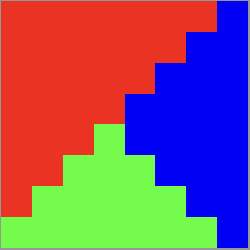
\includegraphics[scale = 0.68]{items/Abbildung1a.png} }}%
        \qquad
        \subfloat{{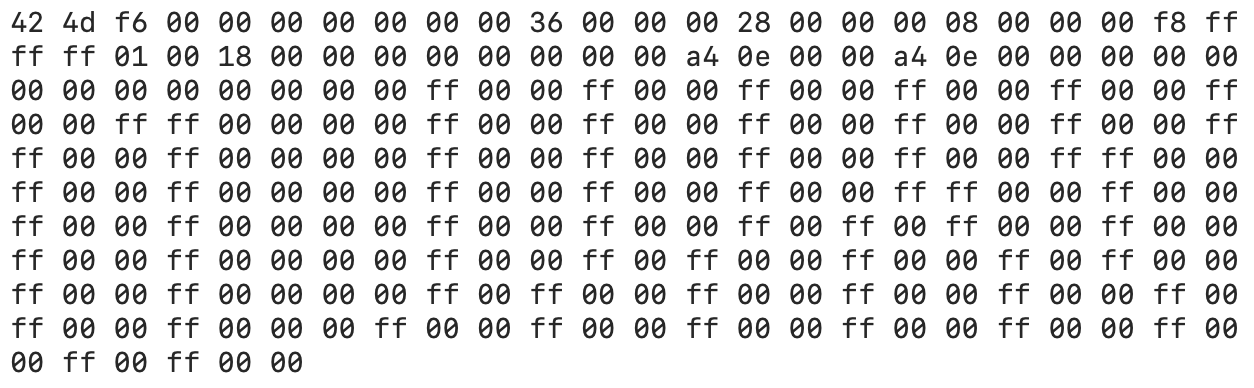
\includegraphics[scale = 0.48]{items/Abbildung1b.png} }}%
        \caption{8x8 Pixelbild mit Top-Down-Ansatz~\cite{SampleBmpFiles}}%
        \label{fig:enter-label}
    \end{figure}

    Das Ergebnis kann in der Abbildung 2 beobachtet werden. Das Programm speichert das resultierende Bild
    in einem Top-Down-Ansatz wobei die Höhe negativ geschrieben wird. Das heißt, dass die erste Zeile des neue erstellten Bildes zuerst im Array geschrieben wird.
    Aus dem Ergebnis kann man klar sehen, dass die Pixelwerte aus dem Ursprungsbild korrekt gelesen und vermehrt sind.

    \begin{figure}[ht]%
        \centering
        \subfloat{{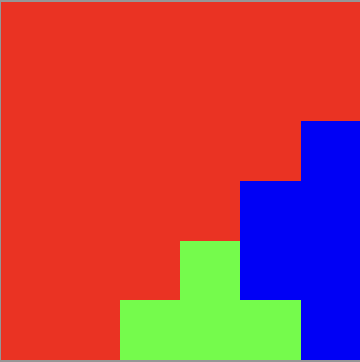
\includegraphics[scale = 0.45]{items/Abbildung2a.png} }}%
        \qquad
        \subfloat{{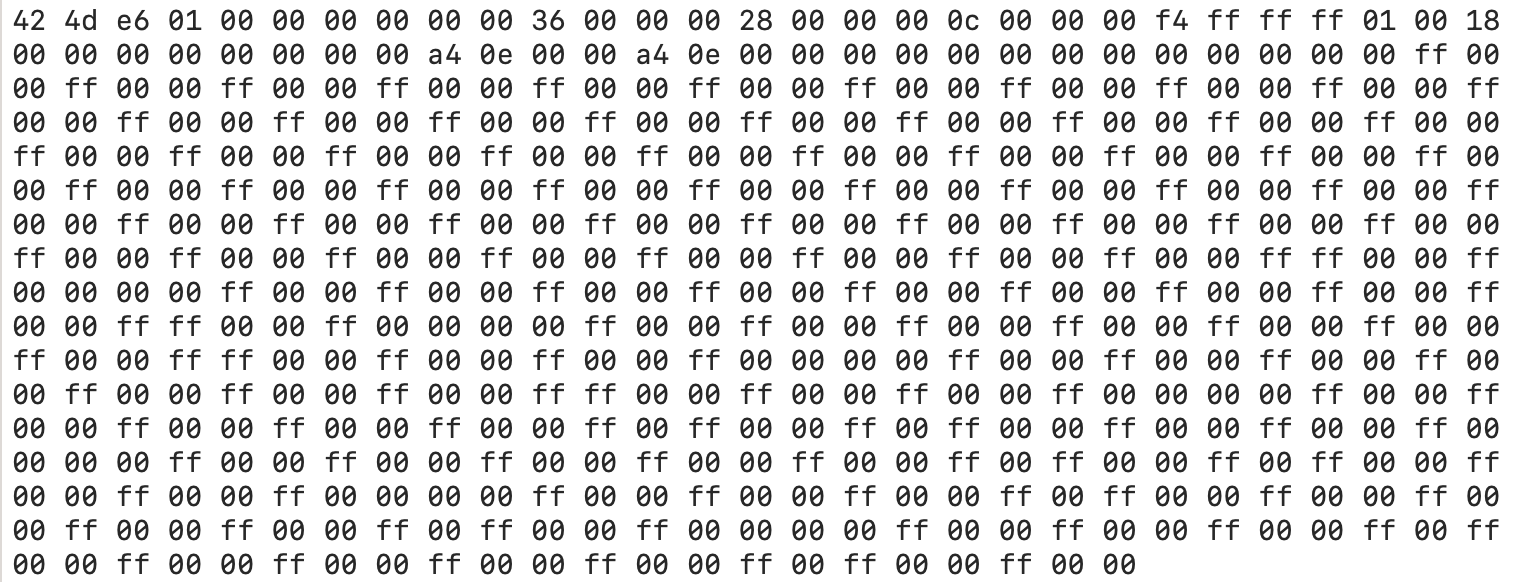
\includegraphics[scale = 0.4]{items/Abbildung2b.png} }}%
        \caption{Ergebnis des ersten Tests}%
        \label{fig:enter-label1}
    \end{figure}

    In einem anderen Beispiel wird das Programm mit dem in der Repository gegebenen Bild lena.bmp getestet.
    Hier geht es um einen 512x512-Pixelbild mit einem Bottom-Up-Ansatz. Der Test prüft ob das Programm beginnend
    mit anderen Koordinaten als der Ursprung -beispielsweise (170,170)- einen Fenster ausschneiden und dies vergrößern
    kann. Ein Fensterausschnitt mit einer Breite von 200 und Höhe von 300 wird in diesem Test ausgeschnitten und um 3
    vergrößert. Das originale Bild sowie das Resultat des Programms ist in der 3. Abbildung zu sehen.

    \begin{figure}[ht]%
        \centering
        \subfloat{{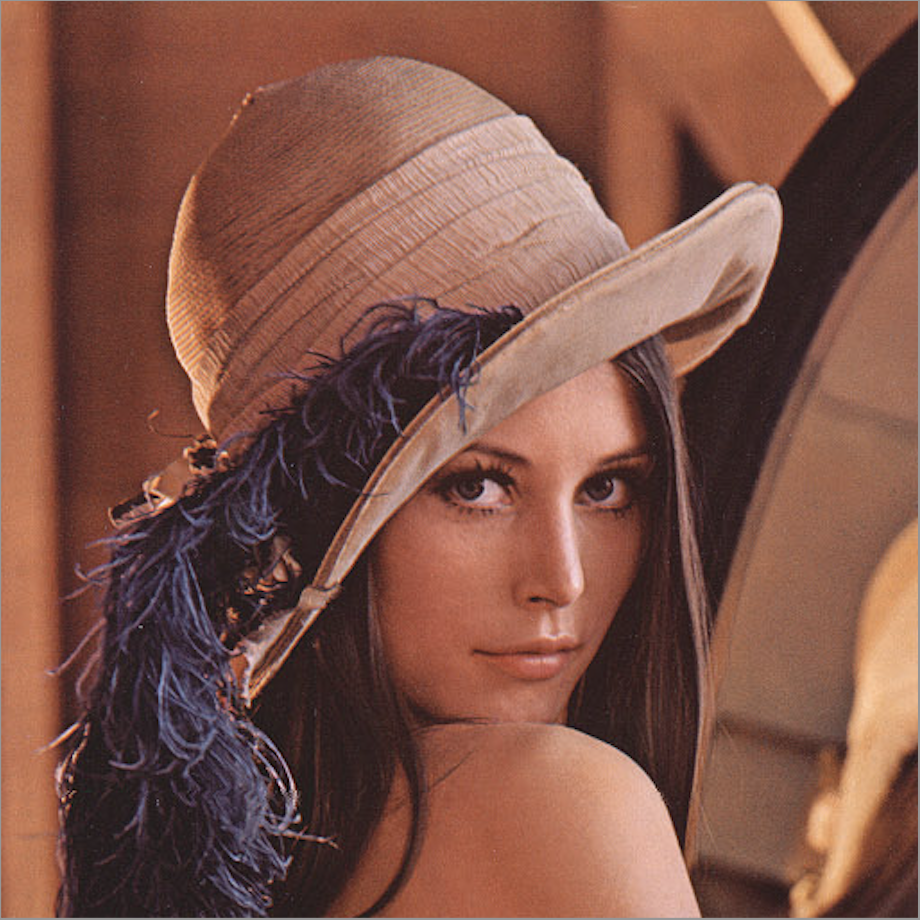
\includegraphics[scale = 0.45]{items/lena.png} }}%
        \qquad
        \subfloat{{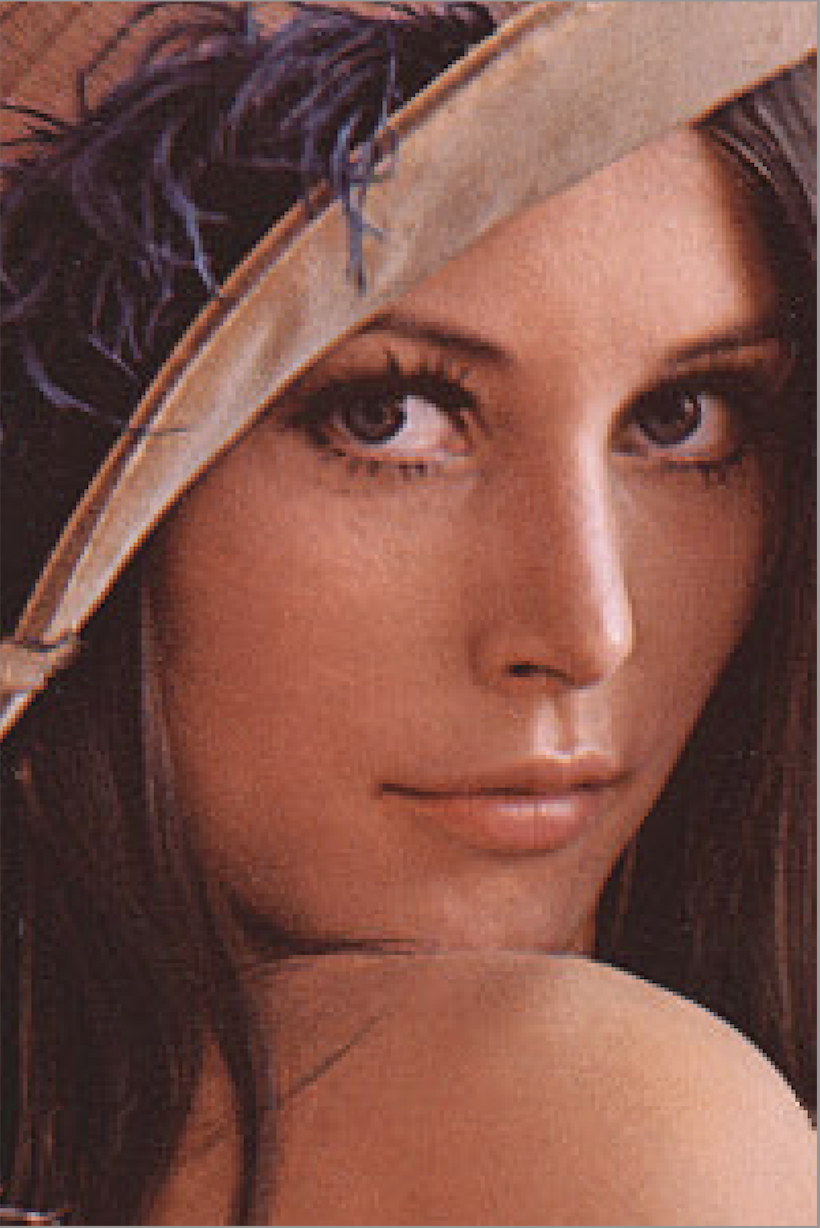
\includegraphics[scale = 0.25]{items/lena-fenster.png} }}%
        \caption{Test bei großer Skalierung}%
        \label{fig:enter-label2}
    \end{figure}

    Für ein anderes Beispiel wird das andere Bild johnmuirtrail.bmp aus der Repository verwendet. Der Test prüft ob das
    Programm ein Fenster ausschneiden und um 2 vergrößern kann, welches eine Breite von 70 und Höhe von 90 hat. Das bedeutet,
    dass das entstandene Pixelbild den 4-Byte-Alignment ohne zusätzliche Null-Bytes nicht erfüllt.
    Hier wird getestet, ob das Programm wirklich die nötigen Bytes für den Alignment des Bilds
    bei dem Aufbau der neuen BMP-Datei hinzufügt. Das Ergebnis des Tests kann in der Abbildung 4 beobachtet werden.

    \begin{figure}[ht]%
        \centering
        \subfloat{{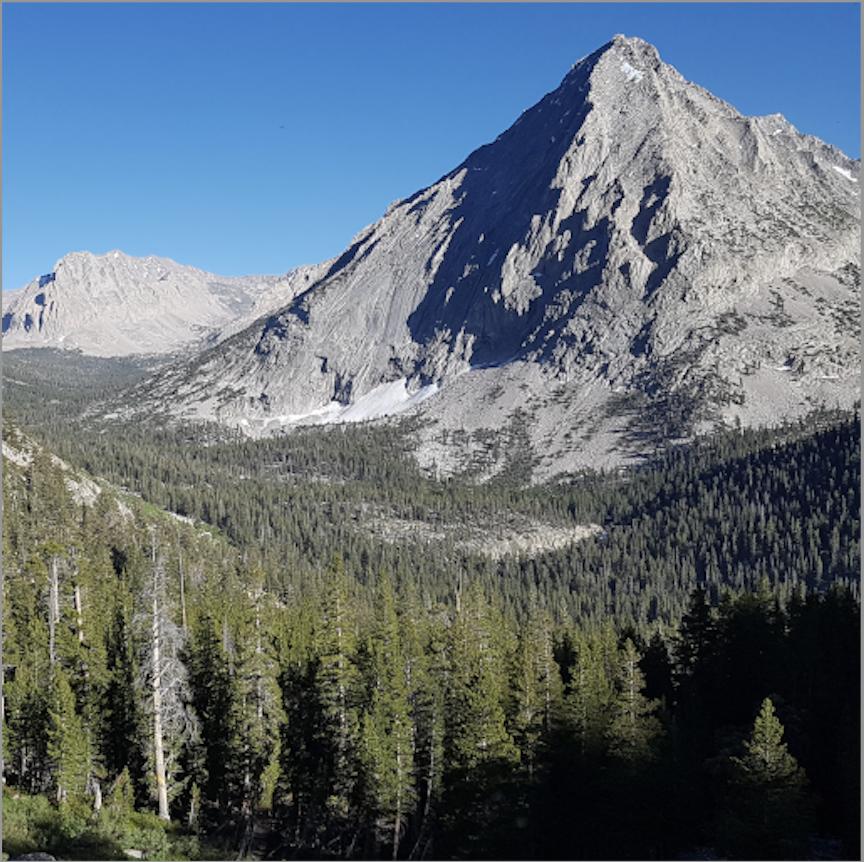
\includegraphics[scale = 0.4]{items/johnmuirtail.png} }}%
        \qquad
        \subfloat{{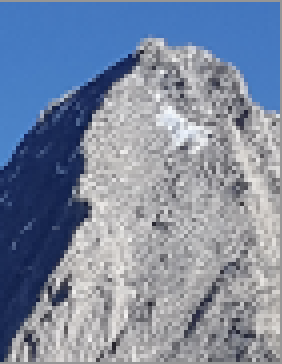
\includegraphics[scale = 0.85]{items/johnmuirtail-fenster.png} }}%
        \caption{Test des 4-Byte-Alignments}%
        \label{fig:enter-label3}
    \end{figure}

    Es gibt auch invalide Eingaben für Koordinaten, Breite und Höhe, Anzahl der Abläufe oder Implementationsoptionen.
    In diesen Fällen werden geeignete Nachrichten über die korrekte Verwendung des Programms ausgegeben. Diese Fällen
    können mit invaliden Eingaben getestet werden.

    \section{Performanzanalyse}

    Die Laufzeit des Algorithmus hängt von der Breite und Höhe des Fensters und dem Skalierungsfaktor ab.
    Die window()-Methode hat die Laufzeitkomplexität $O(width * height)$, da sie $(width * height)$ viele Pixel
    durchläuft und kopiert. Die zoom()-Methode hat auf der anderen Seite eine Laufzeitkomplexität
    von $O(width * height * scale_factor^2)$, da sie die skalierten Pixeldaten ein Mal durchläuft. Also für ein
    gewünschtes nxn-Fenster beträgt die Laufzeitkomplexität des Algorithmus $O(n^2)$.

    Um das Laufzeitverhalten des Programms besser einzuschätzen und die Laufzeiten der Implementierungen zu vergleichen,
    wird die Laufzeit des Programms mit verschiedenen Eingaben gemessen. Diese Messungen finden auf einem System mit einem
    Intel i7-10750H CPU, 2.60 GHz, 16 GB Arbeitsspeicher, Windows 10 Version 22H2, 64-Bit statt. Kompiliert wurde mit
    GCC 8.1.0 (mit MinGW-W64 auf Windows) mit der Optimierungsstufe -O3. Die Berechnung für jede Eingabe wurde 20 mal
    durchgeführt und das arithmetische Mittel davon wurde als Ergebnis mitgenommen.

    Zuerst wird getestet, wie sich die Laufzeit des Programms in Abhängigkeit von der Größe (n x n) des ausgeschnittenen
    Fensters ändert. Dafür wird ein konstanter Skalierungsfaktor von 3 benutzt, wobei für die Breite und Höhe des Fensters
    einen Eingabebereich von 100 bis 3000 benutzt wird.

    \begin{center}
        \begin{tikzpicture}

            \begin{axis}[
                xmin = 0, xmax = 3000,
                ymin = 0, ymax = 4,
                xtick distance = 500,
                ytick distance = 0.5,
                grid = both,
                minor tick num = 1,
                major grid style = {lightgray},
                minor grid style = {lightgray!25},
                width = \textwidth,
                height = 0.5\textwidth,
                xlabel = {Die~Breite~und~Höhe~des~Fensters},
                ylabel = {Laufzeit~in~Sekunden},
                legend cell align = {left},
                legend pos = north west
            ]


                \addplot [blue, mark = *] table [x=x, y=y1, col sep=comma] {items/graph1.csv};
                \addplot [red, mark = square*] table [x=x, y=y2, col sep=comma] {items/graph1.csv};

                \legend{
                    Ohne SIMD (Implementierung 0),
                    Mit SIMD (Implementierung 1)
                }

            \end{axis}

        \end{tikzpicture}
    \end{center}

    Auf dem oberen Graph sind die Laufzeiten von Implementierungen mit und ohne SIMD zu sehen. Beide Kurven steigen quadratisch an,
    wenn die Größe des Fensters sich erhöht. Der Performanzgewinn durch SIMD erhöht sich auch, wenn die Größe des Fensters steigt.
    Zum Beispiel ist bei einem 500x500 Fenster die Implementierung mit SIMD nur ungefähr 0.005 Sekunden schneller als die naive
    Implementierung, aber bei einem 3000x3000 Fenster bringt SIMD einen Speedup von ungefähr 0.165 Sekunden. Der Grund dafür ist,
    dass, wenn die Anzahl der Pixeln sich erhöht, auch mehr Vektorisierung beim Ausschneiden des Fensters stattfindet. Auf der
    anderen Seite ist diese Speedup durch SIMD nur begrenzt, da die zoom()-Methode nicht vektorisierbar ist.

    Es wird auch getestet, wie sich die Laufzeit des Programms in Abhängigkeit vom Skalierungsfaktor ändert. Hierbei wird eine
    BMP-Datei mit einer Größe von 512x512 verwendet, wobei auch das Fenster die Größe 512x512 hat. Der Skalierungsfaktor hat einen
    Eingabebereich von 1 bis 8.

    \begin{center}
        \begin{tikzpicture}

            \begin{axis}[
                xmin = 0, xmax = 8,
                ymin = 0, ymax = 750,
                xtick distance = 1,
                ytick distance = 50,
                grid = both,
                minor tick num = 1,
                major grid style = {lightgray},
                minor grid style = {lightgray!25},
                width = \textwidth,
                height = 0.7\textwidth,
                xlabel = {Der~Skalierungsfaktor},
                ylabel = {Laufzeit~in~Milisekunden},
                legend cell align = {left},
                legend pos = north west
            ]

                \addplot [blue, mark = *] table [x=x, y=y1, col sep=comma] {items/graph2.csv};
                \addplot [red, mark = square*] table [x=x, y=y2, col sep=comma] {items/graph2.csv};

                \legend{
                    Ohne SIMD (Implementierung 0),
                    Mit SIMD (Implementierung 1)
                }

            \end{axis}

        \end{tikzpicture}
    \end{center}

    Auf dem oberen Graph ist es sichtbar, dass die Laufzeit sich quadratisch erhöht, wenn der Skalierungsfaktor ansteigt.
    Die Kurven der SIMD- und naive Implementierung sehen hier sehr ähnlich aus, da der Performanzgewinn mit
    ansteigendem Skalierungsfaktor sich nicht erhöht. Der Grund dafür ist, dass die SIMD-Optimierungen sich beim Ausschneiden
    des Fensters und nicht beim Vergrößern des Fensters befinden. Da die Pixeldatei eine Größe von 512x512 hat, ist der Speedup
    wegen der geringen Vektorisierung niedrig.

    \section{Zusammenfassung und Ausblick}

    Die Aufgabe besteht darin, ein Fenster aus einem unkomprimierten BMP-Bildformat mit 3-Byte-Pixeln auszuschneiden. Dieses Fenster
    wird dann mit Hilfe des Nearest-Neighbor-Algorithmus um einen Skalierungsfaktor vergrößert.

    Das Programm verwendet I/O-Operationen um BMP-Dateien einzulesen, die Daten gewünschtes Fensters der window()-Methode abzugeben,
    das Ergebnis der ersten Operation der zoom()-Methode weiterzuleiten, mit der zoom()-Methode den Fenster zu strecken und als letztes
    wieder eine BMP-Datei aus dem Ergebnis der letzten Operation zu erstellen.

    In der window()-Methode wird ein Algorithmus entwickelt, indem die richtigen Pixelwerten aus der angegebenen BMP-Datei ausgelesen
    und in den resultierenden Pufferspeicher geschrieben werden. Dabei werden sowohl für den Bottom-Up-Ansatz als auch für den Top-Down-Ansatz
    die geeigneten Leseoperationen strukturiert. In der zoom()-Methode werden aus dem Pufferspeicher die Pixeldaten des Fensterausschnitts
    ausgelesen und richtig erweitert.

    Es gibt in dem Programm auch eine andere Implementierungsoption, die eine bessere Leistung als die Naive besitzt.
    In dieser Variante werden Intel Intrinsics bzw. 128-Bit-SIMD-Registern verwendet, indem das Laden und
    Speichern der Pixeldaten optimiert werden.

    Zusammenfassend lässt sich sagen, dass das Programm einen erfolgreichen Algorithmus entwickelt, um die Aufgabenstellung zu
    absolvieren. Der Algorithmus wurde auch verbessert, um eine effiziente Verarbeitung zu gewährleisten. Das Ergebnis des Programms
    ist eine neue BMP-Datei mit dem vergrößerten Fensterausschnitt. Weitere Entwicklungsmöglichkeiten wie SSE-Instruktionen der
    256-Bit-Register können für die Erweiterung des Algorithmus benutzt werden. Verwendung der 256-Bit-Intrinsics erlaubt mehr
    Vektorisierung als 128-Bit-Intrinsics und besitzt bei relativ großeren Eingabebildern eine noch mehr effiziente Performance.
    Da 256-Bit-Intrinsics nicht in SSE4.2 enthalten sind, werden sie in dieser Implementierung nicht verwendet.

% TODO: Fuegen Sie Ihre Quellen der Datei Ausarbeitung.bib hinzu
% Referenzieren Sie diese dann mit \cite{}.
% Beispiel: CR2 ist ein Register der x86-Architektur~\cite{intel2017man}.
    \bibliographystyle{plain}
    \bibliography{Ausarbeitung}{}

\end{document}